

\documentclass[a4paper, 12pt]{article} 
\usepackage{amsmath, amssymb, xcolor, graphicx, enumitem}
\usepackage{fullpage} %smaller margins

%font
%\usepackage[sc]{mathpazo}
%\linespread{1.05}         % Palladio needs more leading (space between lines)
%\usepackage[T1]{fontenc}

%font, libertine
\usepackage{libertine}

%word spacing
\usepackage{microtype}


%useful shortcuts
\def\R{\ensuremath{\mathbb{R}}} %\ensuremath adds math mode, if forgotten
\def\Q{\ensuremath{\mathbb{Q}}}
\def\N{\ensuremath{\mathbb{N}}}
\def\Z{\ensuremath{\mathbb{Z}}}
\def\C{\ensuremath{\mathbb{C}}}

%shorcuts with arguments
\newcommand{\abs}[1]{\left\vert#1\right\vert} %nice absolute values
\newcommand{\bt}[1]{\textbf{#1}} %bold
\newcommand{\eq}[1]{\begin{align*}#1\end{align*}} %aligned equations
\newcommand{\cb}[1]{\centerline{\fbox{#1}}} %centered box
\newcommand{\bp}[1]{\fbox{\parbox{0.8\textwidth}{#1}}} %box paragraph
\newcommand{\norm}[1]{\left\lVert#1\right\rVert} %vector norm
\newcommand{\notimplies}{% does not imply
  \mathrel{{\ooalign{\hidewidth$\not\phantom{=}$\hidewidth\cr$\implies$}}}}
\renewcommand{\eq}[1]{\begin{align*}#1\end{align*}} %aligned equations


%colors
\definecolor{javagreen}{rgb}{0.25,0.5,0.35} %dark green color
\newcommand{\green}[1]{\textcolor{javagreen}{#1}} %command for green
\newcommand{\gray}[1]{\textcolor[gray]{0.5}{#1}} %gray text
\definecolor{blue}{HTML}{268bd2} %blue
\newcommand{\blue}[1]{\textcolor{blue}{#1}} %blue text

%environment
\newcommand{\tab}{\phantom{ssss}}


\title{}
\date{}
%==tips====
%part
    %section, sub, sub
%\begin{enumerate}[resume] %continues counting
\begin{document}
\begin{center}
\section*{Calculus: single}
The Robert Ghrist Approach\\
Mark \\
\end{center}

Relearn

\section{Functions}

%===================e, sin, cos=================================================
\subsection{e, sin, and cos}

Euler's Formula
\cb{
$e^{ix} = \cos(x) + i \sin(x)$ 
}

\gray{for now take as a fact}\\

Define $e^x$ using Taylor as
\eq{
e^x &= 
1 + x + \frac{x^2}{2!} +  \frac{x^2}{2!} +  \frac{x^2}{2!} + \dots\\
& = \sum_{k=0}^\infty \frac{x^k}{k!}.
}


By Euler's Formula, 
\eq{
e^{ix} &= 1 + ix + \frac{(ix)^2}{2!} + \frac{(ix)^3}{3!} + \dots \\
& = 1 - \frac{x^2}{2!} + \frac{x^4}{4!} + \dots 
+ i(x - \frac{x^3}{3!} + \frac{x^5}{5!} - \dots) 
\tag{breaking up real and imaginary} \\
& = \cos(x) + i \sin(x).
}

%===================Taylor=================================================
\subsection{Taylor}
The \bt{Taylor Series} of a function $f$ at $x=0$ is \\
\cb{
$\displaystyle f(x) = f(0) + \frac{f'(0)}{1!}x + \frac{f''(0)}{2!} x^2 + \frac{f'''(0)}{3!}x^3 + \dots$
} \\

*Taylor series can be differented term by term!

\noindent At any other point $a$ it's 
\eq{
f(x) = f(a) + f'(a)(x-a) + \frac{f^{(2)}}{2!}(x-a)^2 + \dots
}
(remember, $a$ must be inside the domain of convergece for the Taylor Poly)

\subsubsection*{Does Taylor exist for every function?}
NO, \textcolor{red}{more on this later}

\bp{
\bt{Geometric Series}
\eq{
1 + r + r^2 + r^3 + r^4 + \dots = \frac{1}{1-r} \tag{for $|r| < 1$}
}
\gray{proof:
$s_n = 1 + r + r^2 + r^3 + \dots + r^n$ \\
Then, $s_n - rs_n = 1 - r^{n+1} \implies s_n = \frac{1-r^{n+1}}{1-r}$ \\
(as $n \rightarrow \infty$, this becomes $\frac{1}{1-r}$ if $|r|<1$)
}
}


\gray{
e.g., 
A neat example is the \bt{Bessel function} used to describe the waves in water when a stone drops: 
\eq{
J_0(x) &= \sum_{k=0}^\infty (-1)^k \frac{x^{2k}}{2^{2k}(k!)^2} \\
& = 1 - \frac{1}{2^2} x^2 + \frac{1}{2^4(2!)^2} x^4 - \frac{1}{2^6(3!)^2} x^6 + \dots
}
note the Bessel function is defined by its Taylor series. \\
It's a decaying cosine-like wave, since the denominator grows faster than cosine's.
}

\graphicspath{{graphs/}}
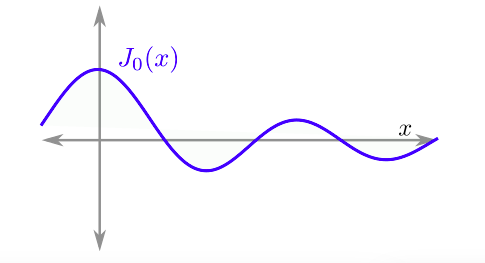
\includegraphics[scale=0.5]{bessel.png}

\subsubsection*{Orders of Growth and Error Size}
\bt{Big-O}: "not faster than" 
\begin{itemize}
    \item f(x) = O(1) if $|f(x)| \leq c*1$ as $x \rightarrow \infty$ (for some c)
    \item f(x) = O(g(x)) if $|f(x)| \leq c*|g(x)|$ as $x\rightarrow \infty$ (for some c)
\end{itemize}
Can be equivalently defined for $x \rightarrow 0$ to describe how quickly a function decays.

\noindent \bt{Little-o}: "ultimately smaller than"
\begin{itemize}
    \item $f(x) = o(g(x))$ means $\displaystyle \frac{f(x)}{g(x)} \rightarrow 0$ as $g(x) \rightarrow 0$.
\end{itemize}


%===================Hyperbolic Trig=================================================
\subsection{Hyperbolic Trigonometric Functions}

These fuctions have similar algebraic properties to $\sin, \cos$ and similarities in their taylor expansions. \\
\gray{(Taylor is the same without alternating signs--all +)}\\
Define 
\eq{
\blue{\sinh(x)} = \frac{e^x - e^{-x}}{2} \\
\textcolor{red}{\cosh(x)} = \frac{e^{x} + e^{-x}}{2} \\
}
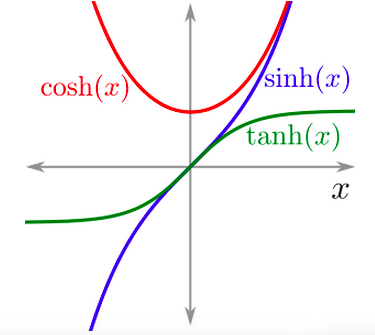
\includegraphics[scale=0.5]{htrig.png}

A variation of the Pythagorean Theorem holds: 
\eq{
\cosh^2(x) - \sinh^2(x) = 1
}

Geometrically, $\cosh$ and $\sinh$ give $x,y$ coordinates on the hyperbola $x^2 - y^2=1$ \\
\tab \tab (similar to $\sin, \cos$ with the unit cirlce).\\

\bp{
\bt{What are hyperbolas?}

They are two parabolas approaching approaching asymptotes (facing up/down or right/left): 
\eq{
\frac{(x-h)^2}{a^2} - \frac{(y-k)^2}{b^2} = 1
}
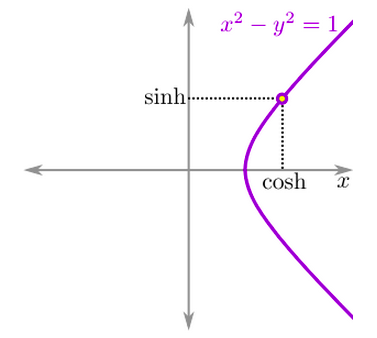
\includegraphics[scale=0.5]{hyperbola.png} \\
(negative sign on x, instead of y, for up/down)
}


%===================Tricks=================================================
\subsection*{\blue{Tricks}}

\blue{
\bt{Multiplying Taylor Polynomials}
\eq{
\cos(x) \cos(x) & = (1 - \frac{1}{2!} x^2 + \frac{1}{4!}x^4 - \dots) (1 - \frac{1}{2!} x^2 + \frac{1}{4!}x^4 - \dots) \\
& = 1 + ( -\frac{1}{2!} - \frac{1}{2!})x^2 + (\frac{1}{4!}+\frac{1}{2!}\frac{1}{2!} + \frac{1}{4!})x^4 + \dots
}
}
\gray{idea: what are the coefficients of $x^4$}

\bp{
\bt{Binomial Series} (for $|x|<1$)
\eq{
(1+x)^\alpha &= 1 + \alpha x + \frac{\alpha(\alpha -1)}{2!} x^2 +  
\frac{\alpha(\alpha-1)(\alpha-2)}{3!} x^3 + \dots \\
& = \sum_{k=0}^\infty \binom{\alpha}{k} x^k.
}
\gray{by computing derivatives and using Taylor Expansion }
}

%===================Exercises=================================================
\subsection*{\green{Exercises}}
\begin{enumerate}
    \item Find the Taylor Expansion of $\ln(1+x)$ using $\ln(1+x) = \int \frac{1}{1+x} \, dx$ and the geometric series.

    \item Similarly find the Taylor Expansion of $\arctan(x)$ using 
    $\arctan(x) = \int \frac{1}{1+x^2} \,dx$ and the geometric series.
\end{enumerate}

Summarizing, using Geometric + Taylor Expansion we have: \\
ONLY FOR $|x|<1$, based on geometric series convergence
\begin{itemize}
    \item $\displaystyle \ln(1+x) = x - \frac{x^2}{2} + \frac{x^3}{3} - \dots$ 
    \item $\displaystyle \arctan(x) = x - \frac{x^3}{3} + \frac{x^5}{5} -
    \frac{x^7}{7} + \dots$ 
\end{itemize}


%========================Limits ========================================

\subsection{Limits}

The limit as $x$ approaches $a$ of $f(x)$ \bt{exists} if for all $x$ close, but NOT equal to $a$, $f(x)$ is close to the value of the limit.

A limit may not exist at a discontinuity, blow-up, or oscillation.

A function is \bt{continuous} at $a$ if $\lim_{x \rightarrow a} f(x) = f(a)$.\\

If $\lim_{x \rightarrow a} f(x) = l$ and $\lim_{x \rightarrow a} g(x) = m$, then
\begin{itemize}
    \item $\displaystyle \lim_{x \rightarrow a}f(x) + g(x) = l + m$
    \item $\displaystyle \lim_{x \rightarrow a} f(x)g(x) = lm.$
    \item "root of a limit" $\displaystyle \lim_{x \rightarrow a} \sqrt[n]{f(x)} 
    = \sqrt[n]{\lim_{x \rightarrow a} f(x)}$.
\end{itemize}

If a function is continuous, then you can evaluate a limit by simply plugging in the value $a$.

\subsection*{\green{Exercises}}

\begin{enumerate}
    \item Evaluate $\displaystyle \lim_{x \rightarrow 0} \frac{\sin(x)}{x}$.
    \gray{
    use Taylor (about x=0), since we are interested in $\sin(x)$ as x approaches 0
    }
\end{enumerate}
\section{Differentiation}

\section{Integration}

\section{Series}

\section*{Curiosities}

\bt{Striling's Approximation}

Gives a good asymptotic (as $n$ gets bigger) approximation for $n!$:\\

\eq{
n! \sim \sqrt{2\pi n} (\frac{n}{e})^n
}
Typically written as $\ln(n!) = n\ln(n) - n + O(\ln(n))$. 
\end{document}

